\documentclass[Modultest/Modultest_main.tex]{subfiles}
\usepackage{xr}

\begin{document}
\section{Modultest af RPI\_IF klassen}\label{sec:RPIIFmodultestbilag}
Til at lave modultest af Rpi klassen bruges noget af gamecontroller klassen, da metoderne setState og setMycolor og setOpponentColor er brugt heri. De vil dog være stubs under denne test blot for at se, at kommunikation over i2c virker, som den skal. Der vil i disse metoder ikke være noget kode udover udskrivning til terminalen via UART, at status er ændret eller farvekoderne for playerside er ændret. 
Klassen er boundary til rpi'en og i2c kommunikationen skulle derfor testes. Dette blev gjort med analog discovery. Den kan nemlig bruges som Master i i2c protokollen og kan både sende og modtage beskeder fra PSoC playerside. Test programmet blev lavet således at funktionen sendCupStatus blev kaldt i mains uendelige for loop, der bliver til dette loop tilføjes et delay på et sekund, så funktionen ikke konstant kaldes. Vi gør det på denne måde for at være sikre på at analog discovery altid har noget at modtage fra PSoC'en. Det første der blev gjort var at sende alle status beskeder, hvorefter farvekoden forsøges sendt. Neden for på figur \ref{fig:analog_beskeder} ses beskederne sendt hvor setState funktionen har sørget for at udskrive til terminalen via uart.
\begin{figure}
    \centering 
    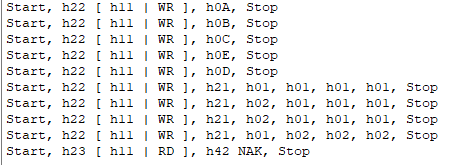
\includegraphics[width=\linewidth]{Modultest/RPI_IF/graphic/analog_beskeder.PNG}
    \caption{De første 5 beskeder er status beskeder til psoc'en, hvor de 4 næste er farvekoden sendt for begge spil sider. Den sidste er ikke noget sendt, men derimod modtaget fra psocen.}
    \label{fig:analog_beskeder}
\end{figure}

Det kan ses at den sidste besked sendt i figuren ovenfor er en besked fra psoc'en sendt til analog discovery. Dette ses tydeligt, da psocen sender en NAK bit tilbage til analog discovery for at fortælle at den ikke har mere data(efter et sekund har den dog igen noget klar på grund af den måde vi har lavet vores test program). Det eneste der ikke blev testet er om interrupt benet går lavt og herefter højt igen hver gang sendCupStatus bliver kaldt. Man kunne godt have gjort dette, men det blev i stedet gjort i integrationstesten mellem raspberry pie og RPI\_IF klassen. Nedenfor i figur \ref{fig:analog_besked} ses et billede af besked nummer 5 sendt i figur \ref{fig:analog_beskeder} fra programmet waveforms, som styrer analog discovery kommunikationen. Man kan se, at der bliver sendt til adressen 11 i hexidecimal tal, hvilket er adressen på i2c slaven. Det er kun denne adresse der skal ændres, når den anden psoc playerside i systemet skal programmeres.
\begin{figure}
    \centering 
    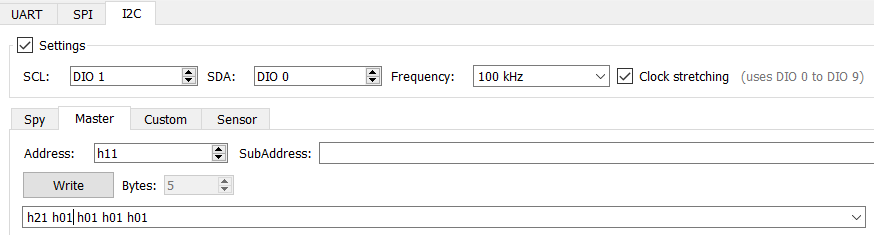
\includegraphics[width=\linewidth]{Modultest/RPI_IF/graphic/analog_besked.PNG}
    \caption{Man ser her en farvekode besked sendt til PSoC'en, hvor playersides egne farve bliver ændret med en farvekode h01 h01 h01.}
    \label{fig:analog_besked}
\end{figure}

\end{document}